\chapter{Persistence}

    \section{I/O devices}

    \sssc{Prototypical System Architecture}

    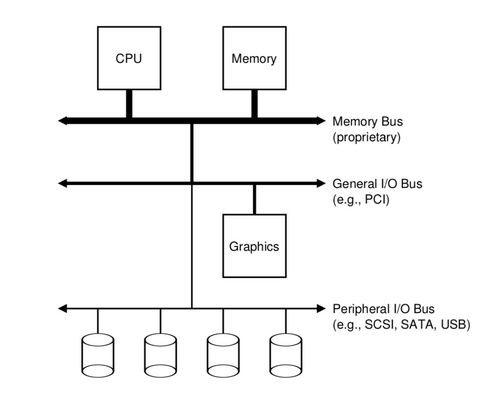
\includegraphics[width=0.6\textwidth]{chapters/Persistence/persistence/psa.png}

    CPU and Memory are connected to the \textbf{Memory Bus}. Other devices like graphic card 
    are connected to the system via a general \textbf{I/O bus}, which should 
    be PCI(or its derivatives). There is even lower bus called \textbf{peripheral bus}, such that 
    \textbf{SCSI,SATA} or \textbf{USB} can be attached here. Those connect slow devices to the 
    system, including disks, mice and keyboards.

    The idea is that: components that demand high performance are nearer the CPU. Lower 
    performance components are further away.


    \sssc{Modern System Architecture}

    Modern systems use specialized chipsets and faster point-to-point interconnects to 
    improve performance.

    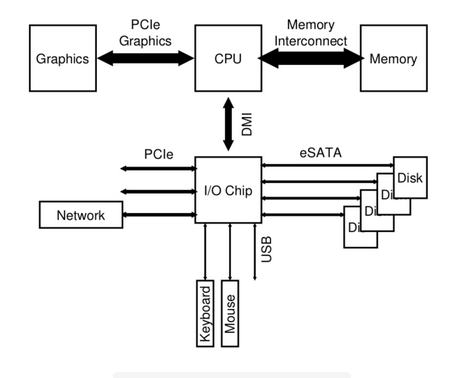
\includegraphics[width=0.6\textwidth]{chapters/Persistence/persistence/msa.png}


    \sssc{Canonical Device}

        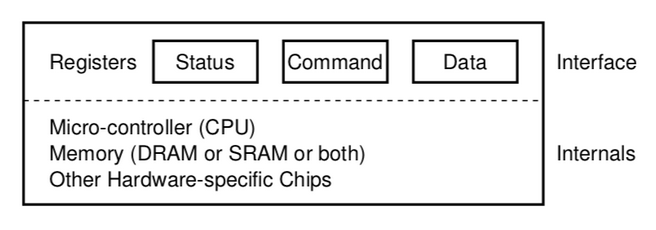
\includegraphics[width=0.5\textwidth]{chapters/Persistence/persistence/canonical_device.png}

        First, each device has its interface to communicate with other device. The interface includes 
        Registers, Buffers.
        
        Second, each device has internal processors/chips to do the processing. Some complex devices 
        may even have CPU and RAM. This internal is also referred as internal. 

    \sssc{Cononical Protocol}

        \begin{enumerate}
            \item Status Register: indicates the current status of the device.
            \item Command Register: to tell device to perform a certain task.
            \item Data Register: pass data to the device or get data from the device.
        \end{enumerate}

        An example of interaction between OS and the device 
        \begin{lstlisting}
            While (STATUS==BUSY)
            ; // wait until the device is not busy

            Write data to DATA register
            Write command to COMMAND register 
                (starts the device and executes the command)

            While (STATUS==BUSY)
            ; // wait until device is done with your request
        \end{lstlisting}


        Although this approach works correctly, it is inefficient. It wastes a great deal of 
        CPU time waiting for the STATUS becomes not busy.
    
    \sssc{Lower CPU overhead with Interrupts}

        Instead of polling the device repeatedly, the OS can issue an request, put the calling process 
        to sleep, and context switch to another task. When the device fulfills the request,
        it raise hardware interrupts to tell the job is done.

        Here is a comparison between polling approach and interrupts approach.

        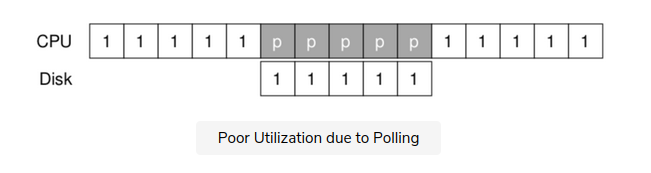
\includegraphics[width=0.6\textwidth]{chapters/Persistence/persistence/poor_polling.png}

        Interrupt approach allows for overlap.

        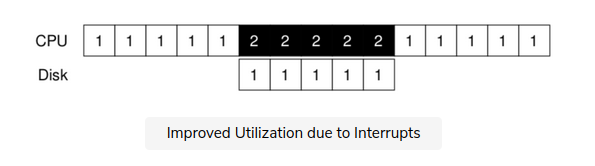
\includegraphics[width=0.6\textwidth]{chapters/Persistence/persistence/improved_interrupts.png}
    
    \sssc{Problem with Interrupts}

    For example, imagine a device that performs its tasks very quickly: 
    the first poll usually finds the device to be done with a task. Using an interrupt, 
    in this case, will actually slow down the system because switching to another process, 
    handling the interrupt, and switching back to the issuing process is expensive. 

    Thus, if a device is fast, it may be best to poll. 
    If it is slow, interrupts, which allow overlap, are best. 

    If the speed of the device is not known, it will be best to use a \textbf{hybrid(two-phased)} 
    that polls for a little while and then, if the device is not yet
    finished, uses interrupts.

    Also, in \underline{networking} or other I/O intensive systems, it is better to avoid 
    interrupts. When a huge stream of incoming packets each generate an interrupt, 
    it is possible for the OS to \textbf{livelock}-only process interrupts.

    \sssc{Coaslescing}

    A device waits for a bit before delivering the interrupt to the CPU $\Rightarrow$ collect 
    more interrupts to handle in one delivery.

    \sssc{DMA: more efficient data movement}

        Suppose, a program wants to write data into disk, it has to copy data from memory 
        to disk DATA explicity, one word at a time. 

        The writing is marked as 'c'.
        
        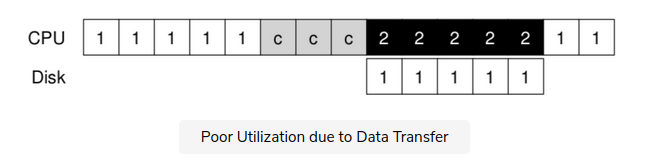
\includegraphics[width=0.6\textwidth]{chapters/Persistence/persistence/poor_write_to_disk.png}


        However, with Direct Memory Access(DMA). The CPU can tell DMA engine where the data exists 
        in the memory, how much data to copy, and which device to send it to. DMA controller will do
        all the write, and issues interrupt when finished.

        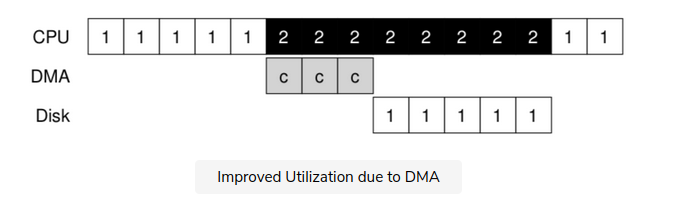
\includegraphics[width=0.6\textwidth]{chapters/Persistence/persistence/improved_by_DMA.png}

    \sssc{Explict I/O instructions}

        On x86, \textbf{in} and \textbf{out} instructions can be used to communicate with 
        specified devices.
        Such instructions are usually \textbf{privileged}.

    \sssc{Memory-mapped I/O}

        With this approach, the hardware makes device registers available as if they were memory 
        locations. To access a particular register, the OS issues a load or store to the address.

    \sssc{Device Driver}

        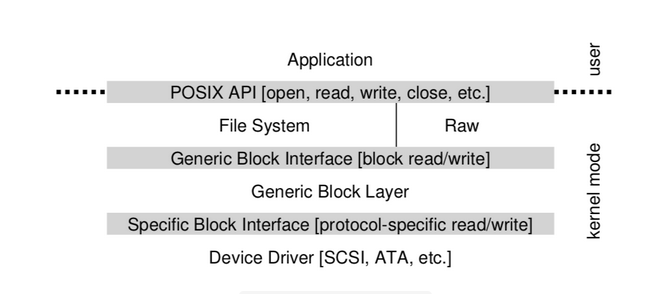
\includegraphics[width=0.6\textwidth]{chapters/Persistence/persistence/Linux_software_organization.png}

        Device driver provide abstraction, and OS can communicate with different devices without 
        knowing detailed implementation.

    \sssc{Problem with device driver}

        \begin{enumerate}
            \item rich features lost in the encapsulation, since uniform is required.
            \item 70 percent of linux kernel reveal is device drivers.
            \item drivers are written by "amateurs"
        \end{enumerate}


\section{Hard Disk Drives}

    \sssc{Interface}

        The drive consists of a large number of sections (512-byte blocks), each can be written 
        or read. Sectors are numbered from 0 to n-1 on a disk with n sectors. Thus, the disk 
        can be viewed an an array of sectores. Disk [n][512].

        One can assume that accessing blocks in a contiguous chunk is fastest access mode.

    \sssc{Seek Time}

        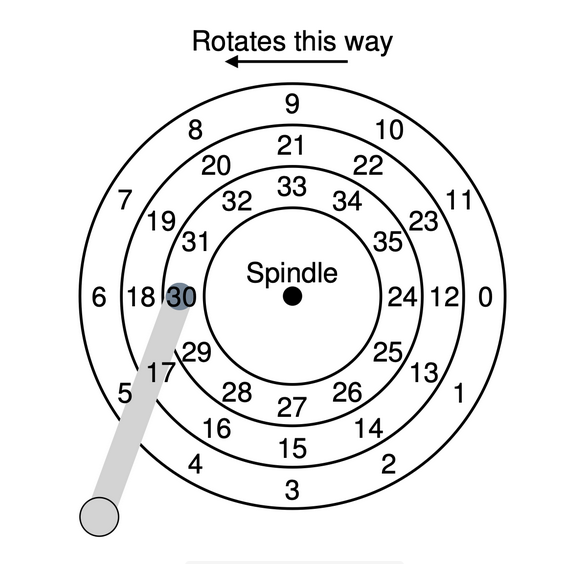
\includegraphics[width=0.6\textwidth]{chapters/Persistence/persistence/tracks.png}

        \textbf{Seek}: move the disk arm to the correct track, very expensive.

        A seek has many phases

        \begin{enumerate}
            \item acceleration phase as the disk arm gets moving.
            \item coasting as the arm is moving at full speed.
            \item deceleration as the arm slows down.
            \item settling as the head is positioned over the correct track.
        \end{enumerate}

        The \textbf{settling time} is quite significant, e.g, 0.5 to 2ms.

        After seeking, we have to wait the sector to pass the head, that is \textbf{rotation delay}.
    
    \sssc{HDD I/O time}

        \begin{equation*}
            T_{I/O} = T_{seek} + T_{rotation} + T_{transfer}
        \end{equation*}

    \sssc{Disk scheduling}

        Unlike CPU scheduling, the job size is known in the disk scheduling. Thus, 
        the scheduler would try to follow the \textbf{principle of SJF} in its operation.

        \begin{enumerate}
            \item SSTF: shortest seek time first. 
            Potiential starvation and seek changes when filfull a request(NBF:nearest-block-first is a makeup).
            \item Elevator(SCAN/C-SCAN): Move head back and forth across the disk, servicing requests 
            in order across the tracks.
            \item SPTF: shortest positioning time first. This depeneds on the seek time and rotation time,
            if the seek time is faster, it favor less rotation. Otherwise, it favors less seeks.
        \end{enumerate}


\ssc{RAID}

        RAID: Redundant Array of Inexpensive Disks.

        Externally, RAID looks just like a disk. Internally, the RAID 
        is complex, consisting of multiple disks, memory, and some processors
        to manage them.

        \textbf{Advantages of RAID}
        \begin{enumerate}
            \item Performance: use multiple disk in parallel can speed up I/O
            \item Capacity
            \item Reliability:  with some redundancy, it would prevent a single point 
            failure.
            \item \textbf{Transparency}: the system sees the RAID as a gigant disk.
        \end{enumerate}


    \sssc{Fault model}

        RAID is designed to detect and recover from certain kinds of disk faults.

        \textbf{The fail-stop fault model}: in this model, disk can either be 
        working or failed.  When a disk has failed, we assume it is permanently lost.

        Assume failed disk can be easily detected.

    \sssc{Evaluation of RAID}

        Three critera
        \begin{enumerate}
            \item Capacity: given N disks with B blocks, how much space is available to clients?
            \item Reliability: how many disk faults that a design can tolerate?
            \item Performance: before evaluating performance, we present a set of typical workloads 
            that one should consider.
        \end{enumerate}

        Three important RAID designs:
        \begin{enumerate}
            \item RAID LEVEL 0 (striping)
            \item RAID LEVEL 1 (mirroring)
            \item RAID LEVEL 4/5 (parity-based redundancy)
        \end{enumerate}

    \sssc{RAID LEVEL 0}

        There is no redundancy at level 0(striping), simply round robin fashion to spread 
        the blocks across the disks.

        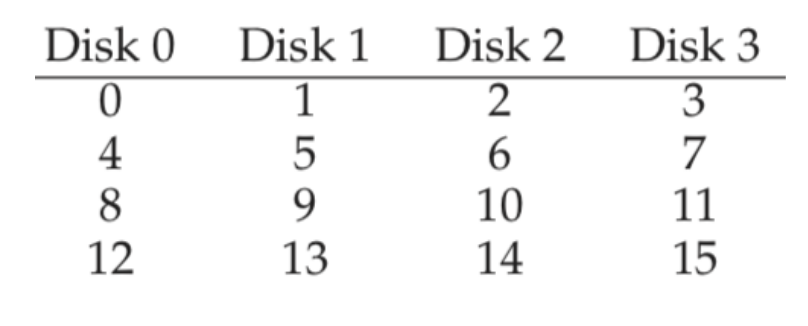
\includegraphics[width=0.5\textwidth]{chapters/Persistence/persistence/level_0.png}

        Evaluation:

        \begin{enumerate}
            \item Perfomance: it is designed to extract most parallelism from array. Sequential workload 
            is way higher than random workload.
            \item Capacity: striping is perfect at this case, 100 percent capacity can be used.
            \item 
        \end{enumerate}

        Throughtput : N*S and N*R

    \sssc{RAID LEVEL 1}

        This is mirroring and get a copy of all the data (in seperate disks) to 
        tolerate disk fault.

        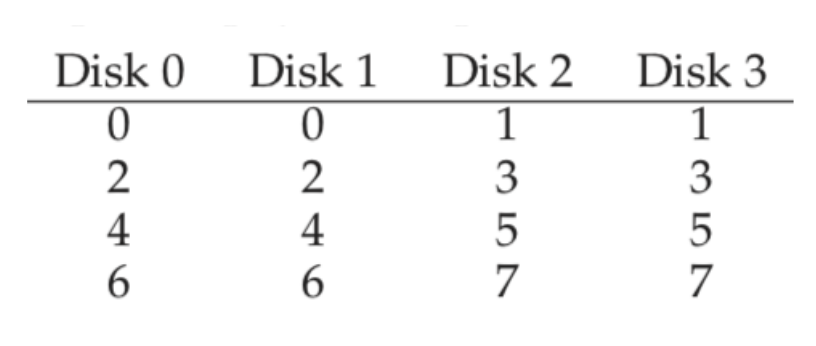
\includegraphics[width=0.5\textwidth]{chapters/Persistence/persistence/level_1.png}

        For read, mirroring can read either copy, but for write, it must update
        contents in both copies.

        \begin{enumerate}
            \item Capacity: The usable capacity for client is (N*B)/2
            \item Reliability: This can tolerate 1 disk failure for certain, and 
            N/2 disk failure by chance.
            \item 
        \end{enumerate}

        Throughtput : N*S/2, N*R/2


    \sssc{RAID LEVEL 4}

        Use \textbf{parity}, we can ensure reliability without huge capacity 
        penalty as mirroring has.

        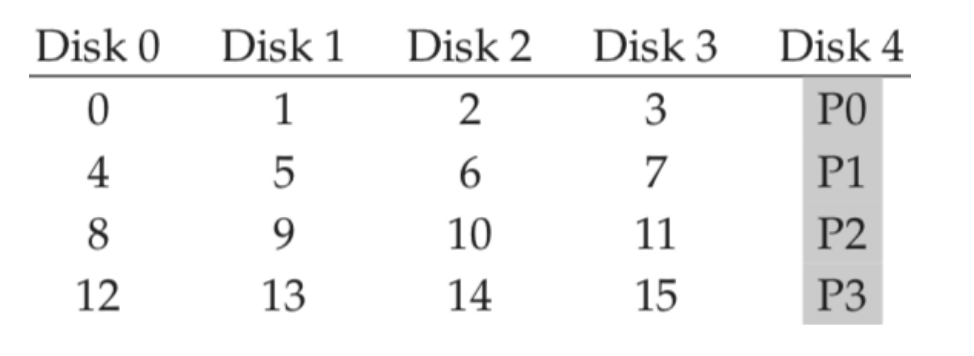
\includegraphics[width=0.5\textwidth]{chapters/Persistence/persistence/level_4.png}

        Use an extra disk 5 to store the parity which is calculated from 
        the striping of disk 1-4.

        It turned out that XOR is excellent parity. Invariant: C1 xor C2 xor C3 xor C4 = P,
        reconstruction: P xor C1 xor C2 xor C3 = C4.


        \begin{enumerate}
            \item Capacity: (N-1)*B
            \item Reliability: It only tolerate a single disk failure.
            \item Performance: (N-1)*R, (N-1)*S
        \end{enumerate}


        However, to maintain the parity is very costly and it is the bottleneck.
        Yes, we can write parallelly in the disk 1-4, but we cannot update the parity 
        parallelly.

    \sssc{RAID LEVEL 5}

        We can use \textbf{Rotating Parity} to address the writing to parity 
        issue.

        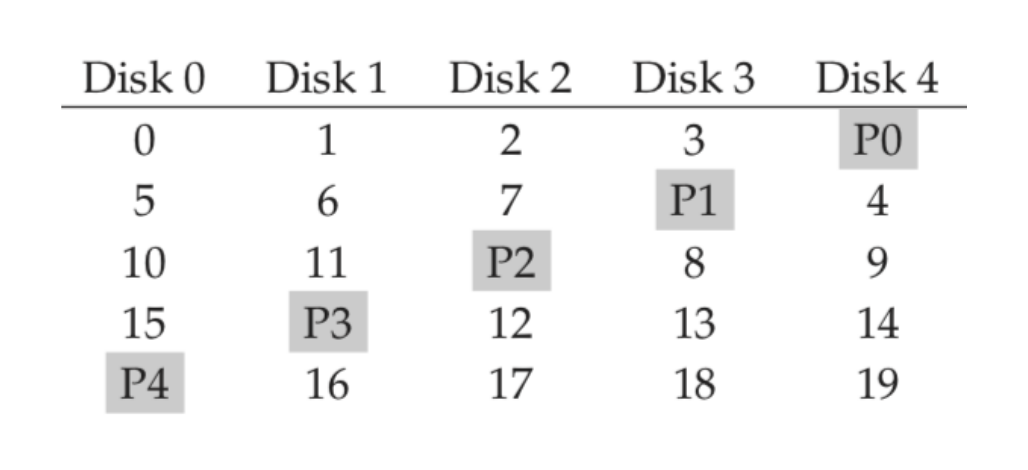
\includegraphics[width=0.5\textwidth]{chapters/Persistence/persistence/level_5.png}


\section{Files and Directories}

        \textbf{File:} linear array of bytes that one can read or write. Each file 
        has a low-level name called inode for historical reason.

        \textbf{Directory:} directory also has a low-level name,
        and it contains a list of pairs $\lbrace \text{file name}, inode \rbrace$,
        $\lbrace \text{directory name}, inode \rbrace$(we can have a directory 
        tree/hierarchy at this case).

    \sssc{The File System Interface}
        
        \begin{lstlisting}
            int fd = open("foo", O_CREAT|O_WRONLY|O_TRUNC,
                        S_IRUSR|S_IWUSR);

            // returns a file descriptor.
        \end{lstlisting}

        A file descriptor is just an integer, private per process, and is used in 
        UNIX systems to access file. Think it as a \underline{capacity}, a 
        handle that gives you the power to perform certain operations.
        Or a pointer to an \underline{object} of type file.

    \sssc{File Descriptors}

        File descriptors 0,1,2 are taken
        \begin{enumerate}
            \item standard input 
            \item standard output 
            \item standard error
        \end{enumerate}

        If a process opens first file, it would certainly be file descriptor 3.

        Each process maintains an array of file descriptors, each of which 
        refers to an entry in the system-wide open file table.
        Each entry in this table tracks which underlying file the descriptor refers to,
         the current offset, 
         and other relevant details such as whether the file is readable or writable.



    \sssc{Read and Write, non-sequentially}

        Each read and write implicitly updates the offset.

        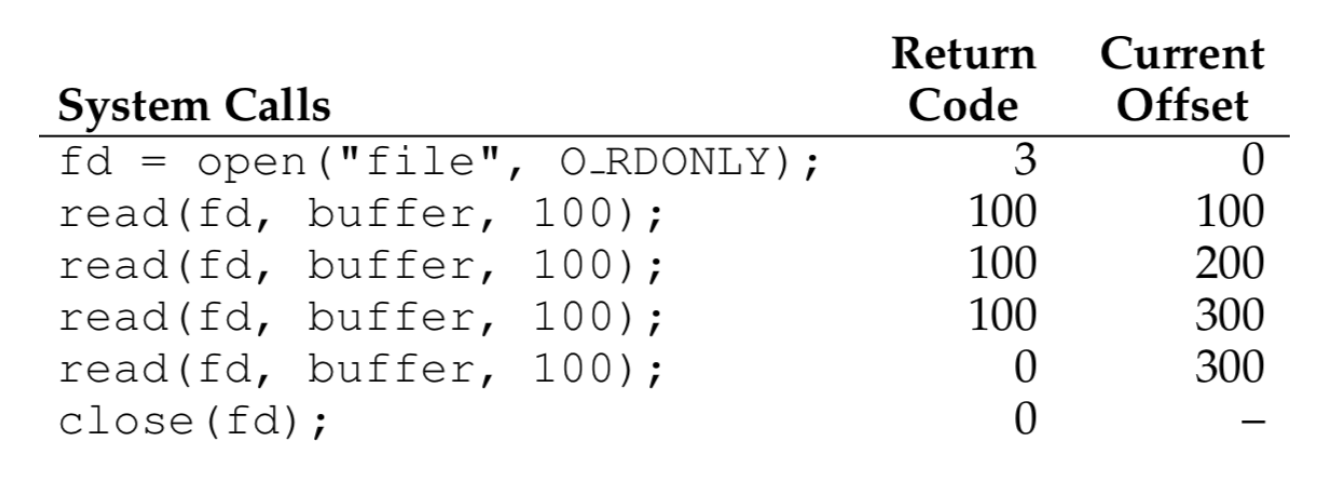
\includegraphics[width=0.5\textwidth]{chapters/Persistence/persistence/use_read.png}


        lseek() explicitly change the offset.

        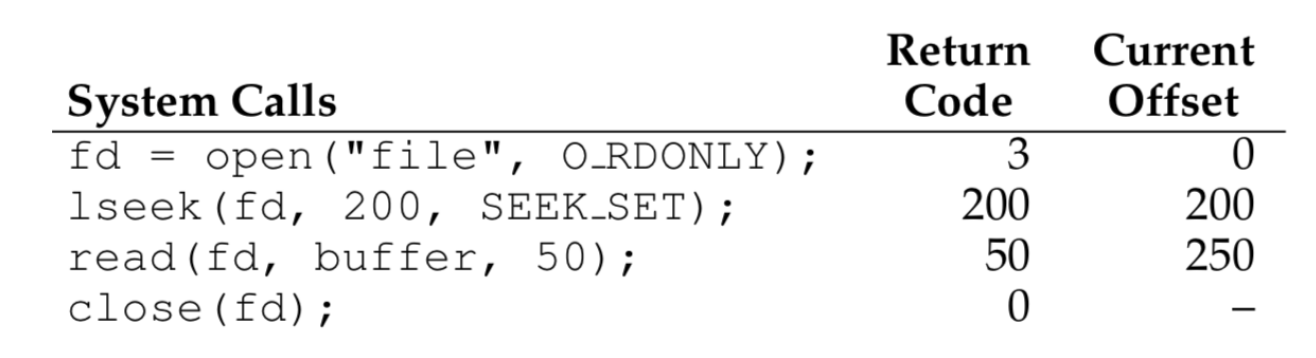
\includegraphics[width=0.5\textwidth]{chapters/Persistence/persistence/lseek.png}


    \begin{lstlisting}
        // only change the offset for the next I/O operation
        off_t lseek(int fildes, off_t offset, int whence);

        /*
            If whence is SEEK_SET, the offset is set to offset bytes.
            If whence is SEEK_CUR, the offset is set to its current
            location plus offset bytes.
            If whence is SEEK_END, the offset is set to the size of
            the file plus offset bytes.
        */


        // stores in the process's structure
        // file table entry
        struct file {
            int ref;
            char readable;
            char writable;
            struct inode *ip;
            uint off;
        };

        // open file table  
        struct {
            struct spinlock lock;
            struct file file[NFILE];
        } ftable;
    \end{lstlisting}

    
    \sssc{Shared File Table Entries: fork() and dup()}

    With fork () the child and parent share the same open file table entry,s
    since they shared the same file descriptor.

    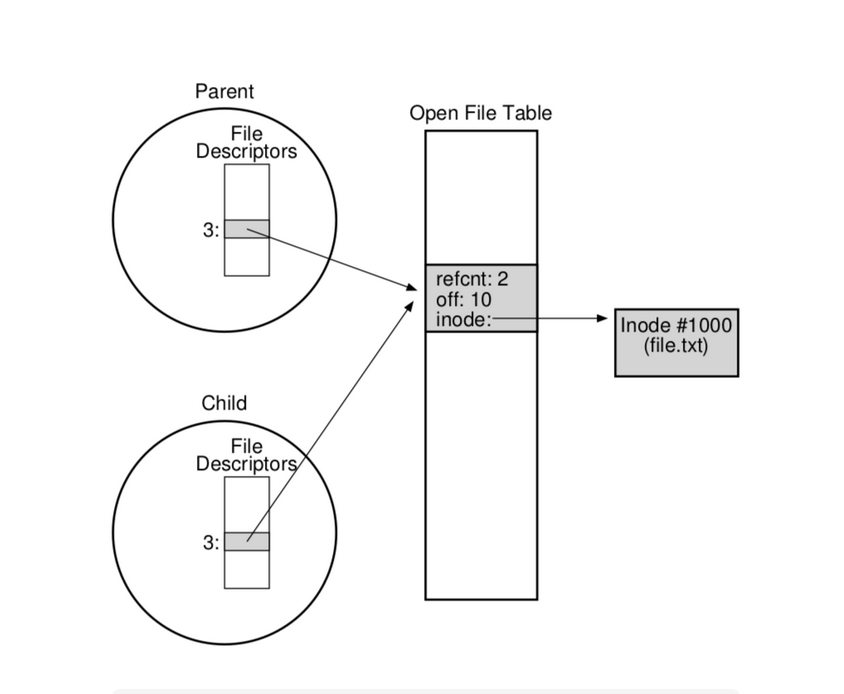
\includegraphics[width=0.5\textwidth]{chapters/Persistence/persistence/share_open_file_table_entry.png}

    Note that there is an \textbf{reference count} in the entry - refcnt.
    When a file table entry is shared, its reference count is incremented,
    only all processes close the file, the entry would be removed.


    Also, there is \textbf{dup()} which allows a process to create a new file descriptor that refers 
    to the same underlying open file as an existing descriptor. Basically copy the file descriptor.


    \sssc{Writing Immediately with fsync()}

    write() only tells the file system to write the data into disk sometimes in the future.
    The system would buffer those writes in memory for perfomance reason.

    For some systems, it is ideal to write data immediately. fsync() is such API that supports the 
    functionality. The fsync() routine returns once all of these writes are complete.

    \begin{lstlisting}
        int fd = open("foo", O_CREAT|O_WRONLY|O_TRUNC,
                S_IRUSR|S_IWUSR);
                assert(fd > -1);
                int rc = write(fd, buffer, size);
                assert(rc == size);
                rc = fsync(fd);
                assert(rc == 0);
    \end{lstlisting}

    The above sequence doesn't guarantee everything that one might expected;
    in some cases, it is required to fsync() the directory that contains foo.
    Because foo might be the newly created file, without this additional 
    fsync(), this might leading to \underline{application-level bugs}.


    \sssc{Renaming Files}

    \begin{lstlisting}
        int fd = open("foo.txt.tmp", O_WRONLY|O_CREAT|O_TRUNC,
                    S_IRUSR|S_IWUSR);
                    write(fd, buffer, size); // write out new version of file
                    fsync(fd);
                    close(fd);

                    // rename the file
                    rename("foo.txt.tmp", "foo.txt");
    \end{lstlisting}

    First, rename() is automic call with respect to system crashes. If the system crashed,
    it would either be renamed the old name or new name.

    \sssc{Metadata of Files}

    \begin{lstlisting}
        struct stat {
            dev_t     st_dev;     //ID of device containing file
            ino_t     st_ino;     //inode number
            mode_t    st_mode;    //protection
            nlink_t   st_nlink;   //number of hard links 
            uid_t     st_uid;     //user ID of owner
            gid_t     st_gid;     //group ID of owner
            dev_t     st_rdev;    //device ID (if special file)
            off_t     st_size;    //total size, in bytes
            blksize_t st_blksize; // blocksize for filesystem I/O
            blkcnt_t  st_blocks;  // number of blocks allocated
            time_t    st_atime;   //time of last access
            time_t    st_mtime;   //time of last modification
            time_t    st_ctime;   //time of last status change 
        };
    \end{lstlisting}

    You should just think of an inode as a persistent data structure kept by the file system 
    that has information like we see above inside of it. 

    All inode reside on disk; a copy of active ones are usually cached in the memory to 
    speed up access.

    \sssc{Removing Files}

        \textbf{unlink()} is the API to remove a file. But why doesn't it called remove() or delete().
        
    \sssc{Making Directories}
        \textbf{mkdir}

    \sssc{Reading and Deleting Directories}

        \textbf{opendir(),readdir(),closedir()}.

        For each directory entry in the readdir(dir).

        \begin{lstlisting}
            struct dirent {
                char d_name[256];         // filename
                ino_t d_ino;              // inode number
                off_t d_off;              // offset to the next dirent
                unsigned short d_reclen;  // length of this record
                unsigned char  d_type;    // type of file
            };
        \end{lstlisting}

        \textbf{rmdir()} has the requirment that the directory be empty.

    \sssc{Hard Link}

        \textbf{link()} creates another name in the directory you are creating the link to,
        and refers it to the same inode number of the original file. It only gives you another 
        file name that refers to the same file.

        \textbf{unlink()} unlinks a file with the inode, and decrease the reference count(link count)
        within the inode. When the reference count reaches zero does the file 
        system also free the inode and related data blocks, and thus truly "deleted" the file.

    \sssc{Symbolic Link}

        Hard links are limited because you cannot create one to a directory.

        Symbolic points to the pathname of file.

    \sssc{Permission Bits and Access Control Lists}

        Unix has the permission bits like "-rw-r--r--". (owner, group, other)


        Access Control Lists specify a list of who can and cannot read a set of files.

    \sssc{Making and Mounting a File System}

    To make a file system, most file systems provide a tool, 
    usually referred to as mkfs (pronounced “make fs”), that performs exactly this task.

    
    However, once such a file system is created, 
    it needs to be made accessible within the uniform file-system tree. 
    This task is achieved via the mount program 
    (which makes the underlying system call mount() to do the real work). 
    What mount does,
    quite simply is take an existing directory as a target mount point 
    and essentially paste a new file system onto the directory tree at that point.

    \ssc{File System Implementation}

        A unreal file system that services for introduction purpose: VSFS (very simple file system).

        To understand a file system, think about two different aspects of them:
        \begin{enumerate}
            \item Data Structure
            \item Access Method
        \end{enumerate}













